\documentclass[11pt]{article}
\usepackage{amsmath,amssymb,booktabs,graphicx,microtype,xcolor,url,capt-of}
\usepackage[letterpaper,margin=1in]{geometry}
\usepackage{placeins}
\emergencystretch=2em
\setlength{\textfloatsep}{14pt plus 3pt minus 3pt}
\setlength{\floatsep}{12pt plus 2pt minus 2pt}
\setlength{\intextsep}{12pt plus 2pt minus 2pt}
\graphicspath{{figures/}}
\newcommand{\wq}{w_q}
\newcommand{\smin}{\sigma_{\min}}
\newcommand{\kappaJ}{\kappa(J)}
\title{Learning When Black-Hole Hair Is Observable:\\Physical Identifiability, Generalization, and Observable Complementarity}
\author{Ariadna Uxue Palomino Ylla\\Nagoya University, Nagoya, Japan\\\texttt{ariadnaepy@gmail.com}}
\date{September 2026}

\begin{document}
\maketitle

\begin{abstract}
High interpolation accuracy does not establish that physical parameters are
identifiable. We study this distinction in a controlled Kiselev black-hole
benchmark with a validated timelike-emitter and three-dimensional null-geodesic
shooting calculation. The forward analysis shows that ringdown is informative
for the deformation amplitude $k$, whereas photon geometry supplies an
independent response direction that resolves much of the state-parameter
$\wq$ degeneracy. Relative to ringdown alone, ringdown plus photon geometry
improves the grid-median minimum singular value by $4.54\times$ and the median
Jacobian condition number by $2.28\times$. In grouped physical interpolation,
the corresponding identifiable-$\wq$ normalized mean absolute error decreases
from 0.309 for ringdown to 0.087 for the combined features. Random splitting is
more optimistic, while four directional extrapolation tests are substantially
harder and split-conformal coverage falls under distribution shift. Photon
geometry also improves recovery under a non-learned nearest-model inverse,
showing that the gain is not architecture-specific. A uniform
161-phase audit gives a typical normalized prediction shift of
$9.48\times10^{-4}$ but exposes catastrophic extrapolation tails. A subsequent
targeted 321-phase audit resolves the remaining forward-feature comparisons,
yet frozen HGB and random-forest tail shifts exceed predeclared robustness
thresholds. Thus the physical complementarity result is supported, but inverse
estimator robustness remains conditional. This study is a theoretical
identifiability benchmark, not an observational constraint.
\end{abstract}

\section{Introduction}
Scientific inverse models can predict accurately for the wrong reason. Repeated
realizations of one physical system can leak across random partitions;
parameters can be locally degenerate even when observables respond strongly;
and a model can interpolate well while failing under extrapolation or small
numerical perturbations. These distinctions matter in black-hole spectroscopy,
where quasinormal frequencies encode compact-object properties but resolving
multiple physical effects remains difficult \cite{dreyer2004spectroscopy,berti2006spectroscopy,bhagwat2019overtones}.

Kiselev spacetimes provide a controlled two-parameter setting. They do not
stand in for a detector likelihood or a generic beyond-Kerr theory. Their value
here is methodological: exact loss of $\wq$ dependence at $k=0$ supplies a known
rank-deficient boundary, while nonzero $k$ permits direct comparison of forward
Jacobian geometry and inverse-learning behavior \cite{kiselev2003quintessence}.

The study complements rapid gravitational-wave inference based on neural
posterior estimation and normalizing flows
\cite{dax2021realtime,green2020autoregressive,gabbard2022cvae,cranmer2020frontier,papamakarios2021normalizing,pacilio2024ringdown}.
Those methods address posterior computation; the present question is whether
the selected forward observables distinguish the parameters in the first
place. This distinction parallels structural and practical identifiability
analysis in dynamical inverse problems \cite{raue2009identifiability,villaverde2019identifiability}.

This work makes four contributions. It (i) evaluates inverse models with
leakage-aware random, grouped, and directional protocols; (ii) validates
timelike and null Kiselev geodesic shooting with explicit failure accounting;
(iii) quantifies physical Jacobian conditioning and observable
complementarity; and (iv) audits uncertainty, noise, learning curves, and
81--161--321 phase-resolution robustness under frozen estimators.

The published JCAP study in Ref.~\cite{palominoylla2026ringdown} supplies the
hairy-black-hole and ringdown framework. The present work adds timelike-emitter
evolution, three-dimensional null-geodesic shooting, photon-geometry
observables, Jacobian identifiability analysis, leakage-aware random, grouped,
and directional evaluation, non-learned inverse baselines, numerical-resolution
audits, and frozen-estimator robustness tests. This boundary distinguishes the
new inverse-learning and physical-shooting study from its theoretical starting
point.

The central narrative rests on three distinctions: sensitivity is not
identifiability, interpolation is not generalization, and forward convergence
is not estimator robustness.

\section{Physical Model and Identifiability Framework}
The static spherical line element is
\begin{align}
 ds^2&=-f(r)dt^2+\frac{dr^2}{f(r)}+r^2d\Omega^2,\\
 f(r)&=1-\frac{2M}{r}-\frac{k}{r^{1+3\wq}}.
\end{align}
We use geometrized units with $M=1$. The dense historical synthetic domain and
the later 121-point physical shooting domain are distinct datasets and are not
mixed. Leading-eikonal ringdown features use the unstable circular null orbit,
with the known limitations of the geodesic--QNM correspondence kept explicit
\cite{cardoso2009geodesic,konoplya2017correspondence,palominoylla2026ringdown}.

For standardized observables $\tilde{\mathbf O}$ and parameters
$\boldsymbol\theta=(k,\wq)$, the local Jacobian is
\begin{equation}
 J_{ij}=\frac{\partial\tilde O_i}{\partial\theta_j}.
\end{equation}
Higher $\smin(J)$ and lower $\kappaJ=\sigma_{\max}/\smin$ are favorable. At
$k=0$, $f(r)$ is Schwarzschild for every $\wq$, so the $\wq$ Jacobian column
vanishes exactly. Nonzero rank away from that boundary does not by itself imply
practical recoverability at finite precision.
The rank-aware historical benchmark that motivated the mature physical
calculation is retained in Appendix~\ref{app:historical} and
Fig.~\ref{fig:boundary}.

Exact $k=0$ rank loss is structural, while small nonzero $k$ produces practical
ill-conditioning at finite precision. The historical proxy experiment
suggested that an additional observable family might improve the weakest
parameter direction; this motivated replacing those proxies with validated
physical shooting observables.

\begin{figure}[tbp]
\centering
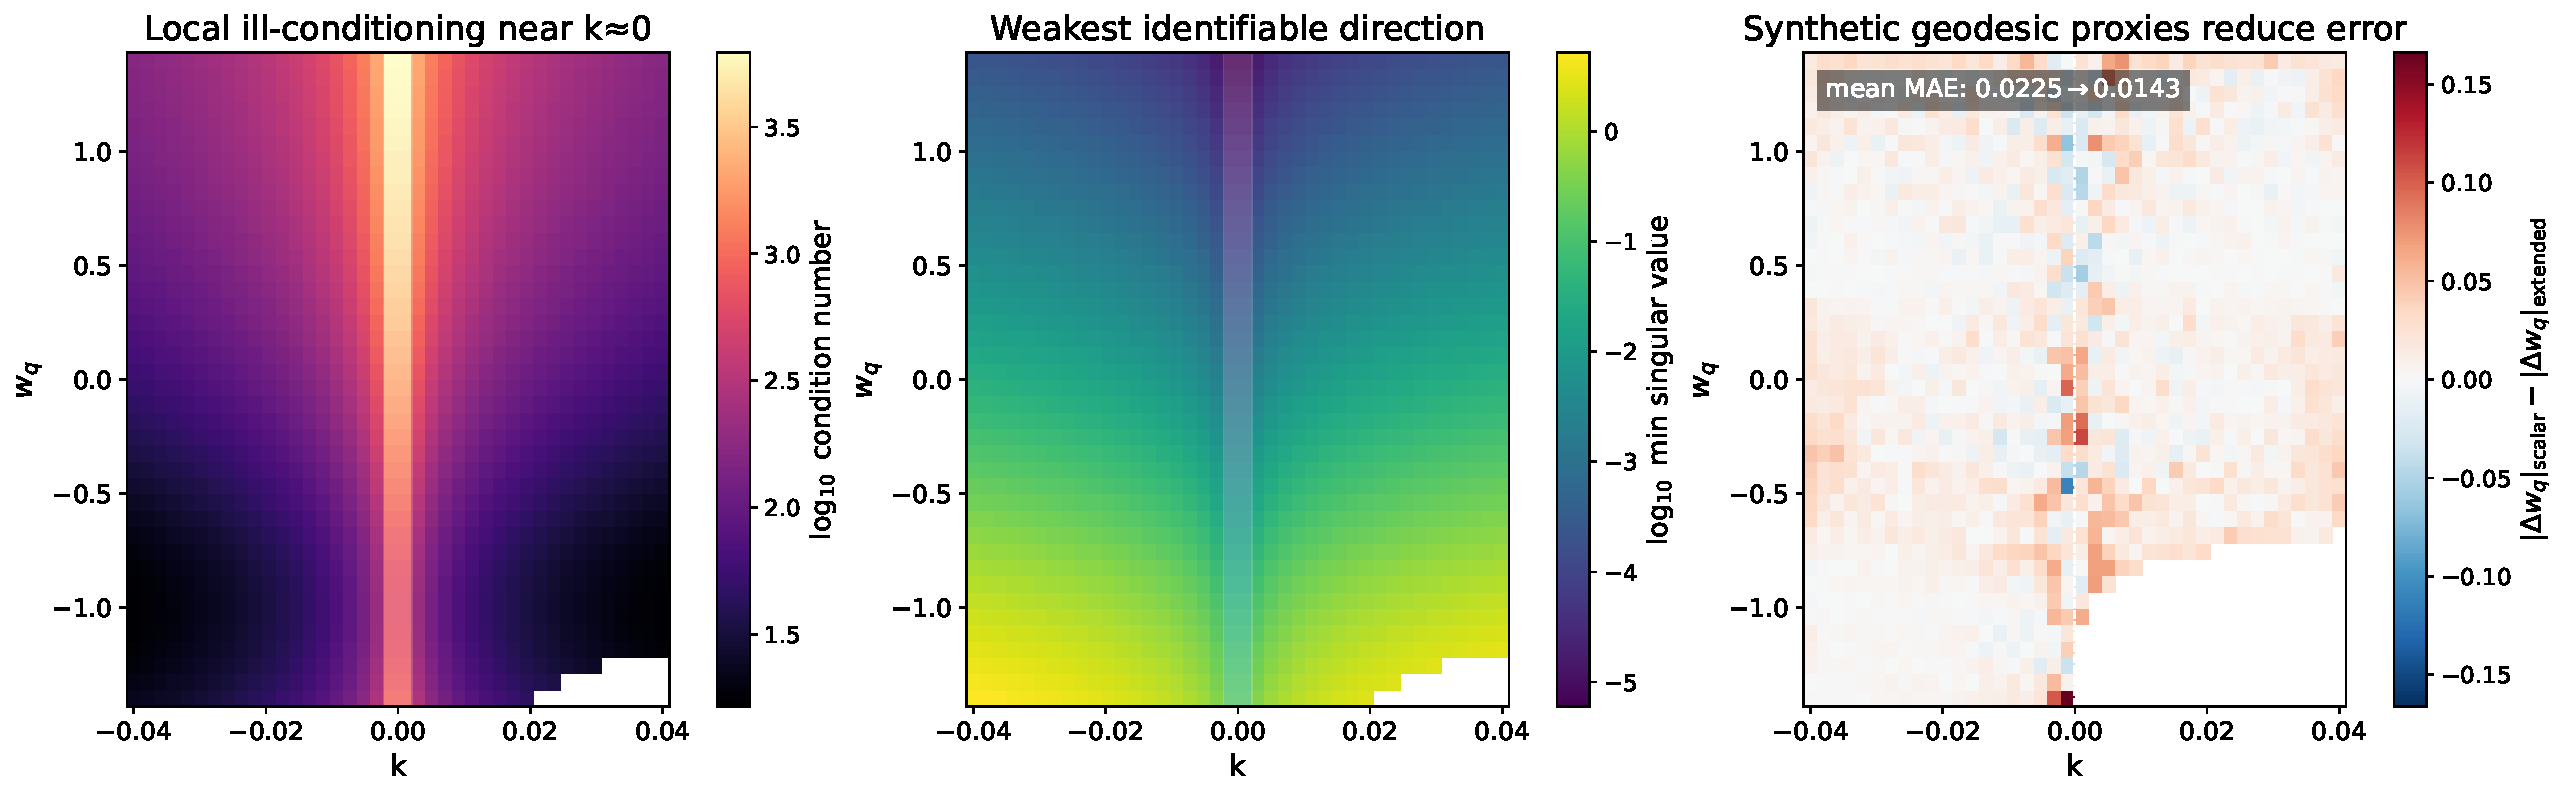
\includegraphics[width=.93\textwidth]{historical_analytic_identifiability_lens.pdf}
\caption{Historical analytic identifiability lens motivating the
physical-shooting study. Left: local Jacobian condition number, which grows
near $k=0$. Center: minimum singular value, showing the weakest identifiable
direction. Right: change in identifiable-$\wq$ error after adding the
historical synthetic geodesic proxies; the mean MAE changes from 0.0225 to
0.0143. White regions are invalid or missing source-grid points and are not
interpolated. The first two panels diagnose inverse-map geometry; the third
records the original proxy experiment and must not be interpreted as physical
ray tracing or geodesic shooting. Proxy augmentation does not resolve the exact
$k=0$ rank loss.}
\label{fig:lens}
\end{figure}

The third panel is therefore historical motivation rather than evidence from
the mature physical solver. The physical results below use timelike-emitter and
three-dimensional null-geodesic integrations without proxy substitution.

\section{Physical Geodesic Shooting and Numerical Validation}
The emitter follows the equatorial timelike Hamiltonian
\begin{equation}
 H=\tfrac12[-E^2/f+fp_r^2+L^2/r^2]=-\tfrac12.
\end{equation}
Its physical coordinate azimuth begins at apocentre:
$\phi=\pi$, $r=r_a$, $p_r=t=\tau=0$. Coordinate $\phi$ is not treated as a
radial anomaly; turning points are detected from $p_r=0$ and the radial
azimuthal period includes apsidal advance.

Photons are propagated in Cartesian spatial coordinates with covariant momentum
$\mathbf p$ and $p_t=-1$,
\begin{equation}
 H_\gamma=\tfrac12[-1/f+\mathbf p^2+(f-1)(\mathbf n\!\cdot\!\mathbf p)^2]=0.
\end{equation}
Two launch angles are solved so the direct branch reaches the observer plane.
The implementation reports failed phases rather than interpolating them or
substituting synthetic geodesic proxies. Photon momenta are projected onto the
static observer tetrad before sky angles are formed. Redshift uses
$1+z=\omega_{\rm emit}/\omega_{\rm obs}$, and direct arrival time is compared
with $\int(1+z)d\tau_{\rm emit}$ after removing one common additive constant.
For clarity, the reported propagation time is
$t_{\rm prop}=t_{\rm hit}-t_{\rm emit}$, and the excess delay removes the
corresponding Euclidean source--observer distance,
$\Delta t_{\rm excess}=t_{\rm prop}-\lVert\mathbf{x}_{\rm obs}-
\mathbf{x}_{\rm emit}\rVert$.  Relative arrival time is expressed on the
static observer's clock as
$T_{\rm rel}=\sqrt{f_{\rm obs}}[(t_{\rm emit}+t_{\rm prop})-
(t_{\rm emit}+t_{\rm prop})_{\rm ref}]$.  The separately reported
$T_z=\int_{\tau_{\rm ref}}^{\tau}(1+z)\,d\tau_{\rm emit}$
(\texttt{toa\_from\_redshift}) is an independent validation quantity obtained
by cumulative trapezoidal integration, not a replacement for $T_{\rm rel}$.

An independently implemented reference solver, which imports no production
\texttt{bhhairml} physics code, verified the metric and derivative (including
explicit $M$ dependence), timelike Hamiltonian and turning-point constants,
Cartesian null Hamiltonian and photon initialization, static-observer tetrad,
redshift, impact parameter, signed sky coordinates, propagation and arrival
timing, physical feature extraction, and selected Jacobians. The maximum
trajectory/observable, full feature-vector, and selected-Jacobian absolute
differences were $7.633557254893203\times10^{-9}$,
$7.774758614687016\times10^{-11}$, and
$2.617905892066119\times10^{-13}$, respectively.

In the Schwarzschild benchmark, all 161 phases succeed for both tested nominal
$\wq$ values, which agree because $k=0$. The independent radial benchmark
validates the turning-point period and apsidal advance. The physical 121-point
grid also preserves the Hamiltonian constraints and exact rank-loss boundary.
The overlapping arrival-time phase-resolved series and their numerical residuals are retained as
supporting evidence in Appendix~\ref{app:numerical-thresholds} and
Fig.~\ref{fig:schwarzschild}.

Figure~\ref{fig:rays} makes the direct-branch geometry explicit using actual
validated emitter states, launch angles, photon integrations, and observer
geometry. It is a controlled benchmark visualization, not a radiative-transfer
or detector simulation.

\begin{figure}[tbp]
\centering
\includegraphics[width=.78\textwidth]{shooting/phase_coloured_photon_shooting_horizontal.pdf}
\caption{Representative direct-branch null geodesics for $M=1$, $r_p=8M$,
$r_a=12M$, $k=10^{-3}$, $w_q=-0.5$, and observer $(0,0,-80M)$. Physical phase
runs from $\pi$ at apocentre to $3\pi$; the diamond marks the numerically
detected pericentre and the dark disk is a horizon-scale marker, not a shadow.
At each phase, two launch angles are solved until the ray reaches the observer.
The right panel shows the stated near-hole coordinate bounds on their actual
scale; no trajectory is geometrically magnified. This is a controlled
dimensionless benchmark.}
\label{fig:rays}
\end{figure}

\section{Physical Observable Complementarity}
A large response can reveal that the spacetime changed without revealing which
parameter caused the change. Timing and redshift responses are often large but
nearly collinear in parameter space. Photon geometry rotates the sensitivity
direction and therefore contributes information that ringdown lacks.
Figure~\ref{fig:shooting-observables} first shows how the same three validated
spacetimes produce distinct phase-resolved response patterns.

\begin{figure}[tbp]
\centering
\includegraphics[width=.88\textwidth]{shooting/shooting_observables_vs_phase_refined.pdf}
\caption{Physical direct-branch observables over $\phi\in[\pi,3\pi]$ for
Schwarzschild and $k=10^{-3}$ with $w_q=-0.5,-2/3$, using $M=1$,
$r_p=8M$, $r_a=12M$, and observer $(0,0,-80M)$. The dashed line marks the
initial apocentre and diamonds mark numerical pericentres. All phase-resolved series use the
same successful matched phases without interpolation. Observable response
amplitude and independent parameter information are not equivalent.}
\label{fig:shooting-observables}
\end{figure}

The standardized local comparison is shown in Fig.~\ref{fig:local}.

\begin{figure}[tbp]
\centering
\includegraphics[width=.78\textwidth]{physical_local_sensitivity_comparison.pdf}
\caption{Local standardized response and separation diagnostics. Timing has a
large response but an angle of $178.76^\circ$ and condition number 1275.5;
photon geometry rotates the response to $159.37^\circ$ and lowers the condition
number to 81.4. Higher $\sigma_{\min}$, angles farther from $180^\circ$, and
lower condition number are favorable; magnitude alone is not identifiability.}
\label{fig:local}
\end{figure}

The full observer tracks nearly overlap, as expected for these small
deformations. Figure~\ref{fig:sky-residuals} therefore retains the physical
track as the primary object and shows unnormalized, pointwise matched-phase
residuals relative to Schwarzschild. These small resolved changes supply a
direction that is difficult to see on the full track.

\begin{figure}[tbp]
\centering
\includegraphics[width=.78\textwidth]{shooting/observer_sky_track_with_residuals.pdf}
\caption{Static-observer-tetrad sky tracks and actual-scale residuals for the
same $M=1$, $r_p=8M$, $r_a=12M$, observer $(0,0,-80M)$ direct-branch benchmark.
Open circles mark $\phi=\pi$ apocentre, diamonds mark numerical pericentre, and
the arrow gives increasing phase. Residuals are pointwise differences from
Schwarzschild at exactly matched successful phases; they are neither
normalized for visibility nor interpolated across failures.}
\label{fig:sky-residuals}
\end{figure}

Using the nominal 81-phase Jacobian archive across the accepted physical grid,
ringdown plus photon geometry improves the
median $\smin$ by $4.5429\times$ and the median condition number by
$2.2819\times$ relative to ringdown alone. The medians for the combined set are
$\smin=1.2326$ and $\kappaJ=4.0731$. Ringdown plus all shooting has
$\smin=1.5312$ and $\kappaJ=4.4974$: adding more responsive summaries can raise
$\smin$ without producing the best conditioning.
The separate 161-phase resolution audit gives, respectively,
$(\smin,\kappaJ)=(1.2326,4.0733)$ and $(1.5319,4.4957)$ for these two
combined sets, confirming that the published nominal-resolution summaries are
stable without changing their provenance.
Figures~\ref{fig:grid} and \ref{fig:complementarity} show the pointwise maps and
their grid-wide summaries, respectively.

\begin{figure}[tbp]
\centering
\includegraphics[width=.97\textwidth]{physical_grid_minimum_singular_value.png}
\caption{Grid maps of $\log_{10}\smin$ with exact $k=0$ rank-loss points
masked. Missing or invalid values are not interpolated, and all panels use one
finite-$k$ color scale.}
\label{fig:grid}
\end{figure}

\begin{figure}[tbp]
\centering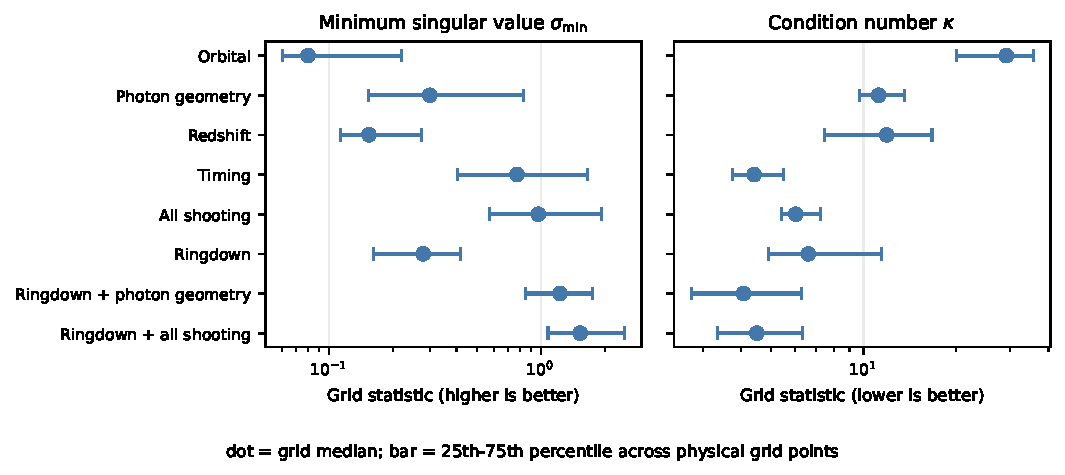
\includegraphics[width=.74\textwidth]{physical_observable_complementarity_landscape.pdf}
\caption{Nominal 81-phase grid-wide median and interquartile summaries of
$\smin$ and condition number. Photon geometry provides the clearest complement
to ringdown; the separate 161-phase audit is reported in the text.}
\label{fig:complementarity}
\end{figure}

\begin{figure}[tbp]
\captionof{table}{Primary physical-complementarity summaries from the nominal
81-phase Jacobian archive. The reported combined-set gains are the archived
grid-wide improvement statistics relative to ringdown, not ratios formed from
separately reported medians; the 161-phase audit values are stated in the text.}
\label{tab:complementarity}
\centering
\scriptsize
\setlength{\tabcolsep}{2pt}
\begin{tabular}{lccc}
Features & med. $\smin$ & med. $\kappaJ$ & gain \\
\hline
Ringdown & 0.2782 & 6.6112 & reference \\
Rdown + photon geom. & 1.2326 & 4.0731 & $4.54\times/2.28\times$ \\
Rdown + all shooting & 1.5312 & 4.4974 & -- \\
\end{tabular}
\end{figure}

\subsection{Finite-domain ambiguity check}
Because local Jacobian rank does not establish global injectivity, we also
tested the sampled physical domain for distant observable near-collisions.
Across all 121 accepted physical points, no finite-$k$ system had a nearest
observable neighbor farther than $d_\theta=0.25$ in normalized parameter
space, and no pair with $d_\theta\geq0.25$ fell below the fifth-percentile
local observable spacing. For ringdown plus photon geometry, the closest pair
with $d_\theta\geq0.5$ has RMS standardized observable distance 0.03155. This
is approximately 12.8 times the largest measured 161-to-321 combined-feature
RMS forward-resolution change, 0.002462.

At $d_\theta\geq0.5$, photon geometry reduces the number of distant pairs
below local-median observable spacing from 13 to 6, increases the closest-pair
distance from 0.02517 to 0.03155, and decreases the maximum
nearest-observable-neighbor parameter distance from 0.23216 to 0.21886. It
therefore reduces the most distant sampled ambiguities. It does not preserve
every local nearest-neighbor ordering and rearranges some nearby systems in
observable space, even while improving the more consequential distant sampled
separation. Full
finite-grid results and limitations appear in Appendix~\ref{app:ambiguity}.

\section{Leakage-Aware Inverse-Learning Protocols}
Five primary feature sets are ordered consistently: ringdown, photon geometry,
all shooting, ringdown plus photon geometry, and ringdown plus all shooting.
Here photon geometry and the other integrated quantities are physical shooting
observables, distinct from the historical synthetic geodesic proxies.
Models are histogram gradient boosting (HGB), random forest (RF), and a
target-scaled multilayer perceptron (MLP) \cite{breiman2001random,friedman2001greedy,pedregosa2011scikit}.
These heterogeneous standard estimators are retained intentionally rather than
optimizing one high-capacity architecture: tree models expose piecewise
split-crossing behavior, while the MLP supplies a smoother perturbation
response and a distinct extrapolation failure mode. Their purpose is to reveal
estimator-specific behavior, not to claim that standard models are universally
preferable.
The protocols are random interpolation, two blocked $3\times3$ grouped physical
layouts, and four directional extrapolation tests. All nominal $k=0$ records
are retained and flagged, but ordinary $\wq$ error excludes them because $\wq$
is exactly non-identifiable there.

Normalized mean absolute error divides MAE by the full target span.
Split-conformal intervals target 90\% coverage and are interpreted under their
exchangeability assumptions \cite{vovk2005conformal,tibshirani2019covariate,angelopoulos2021guide}.
Feature-noise scales and every preprocessing transform are learned on training
folds. The 81-to-161 and targeted 161-to-321 comparisons apply archived frozen
estimators; they do not retrain on higher-resolution test features.

\section{Inverse-Learning Results}
Random splitting is optimistic. For HGB, RF, and MLP considered together,
random ringdown NMAE is 0.0361/0.1688 for $k$/identifiable $\wq$, while grouped
ringdown is 0.0485/0.3093. Ringdown plus photon geometry gives grouped
0.0457/0.0875, with the $\wq$ improvement reproduced independently in both
tree families. Directional extrapolation remains harder: the combined set has
aggregate NMAE 0.1305/0.2012.
Figure~\ref{fig:protocols} compares the three validation regimes directly.

\begin{figure}[tbp]
\centering
\includegraphics[width=.84\textwidth]{physical_ml_protocol_comparison.png}
\caption{Median NMAE for the five primary feature sets under random, grouped
physical interpolation, and directional extrapolation. Directions remain
separate in the machine-readable source before aggregation.}
\label{fig:protocols}
\end{figure}

\subsection{Traditional inverse baselines}
To separate physical complementarity from architecture-specific learning, we
evaluate two non-learned inversions under exactly the same registered physical
holdouts. The nearest physical model fits a standardization transform on the
training observables only, computes every Euclidean distance to the training
catalog explicitly, and returns the $(k,\wq)$ pair of the nearest training
system. The local Jacobian inverse selects its reference from the training
catalog, constructs a training-only local linear forward map, and applies the
Moore--Penrose pseudoinverse. Calibration and test systems participate in
neither construction.

For the nearest baseline, identifiable-$\wq$ NMAE decreases from 0.123810 to
0.086580 under random interpolation, from 0.220833 to 0.148148 under grouped
interpolation, and from 0.254161 to 0.195026 under directional extrapolation
when photon geometry is added to ringdown. These are reductions of 30.1\%,
32.9\%, and 23.3\%, respectively. Observable complementarity is therefore a
property of the physical forward map rather than merely an effect learned by a
particular estimator; nearest-neighbor inversion is not asserted to be
optimal.

For ringdown plus photon geometry, the local Jacobian median
$k$/identifiable-$\wq$ NMAE is 0.0147/0.0259, 0.0184/0.0454, and 0.0661/0.1172 for random,
grouped, and directional protocols. However, 1315 of 9950 raw predictions lie
outside the registered physical domain and were not clipped. Thus strong local
inversion performance coexists with poor global robustness; favorable median
local-linear performance does not establish a reliable global inverse. The
full method comparison is shown in Fig.~\ref{fig:mljac}, with detailed values
and conditioning associations retained in Appendix~\ref{app:traditional}.

Conditioning and coverage explain different aspects of error. In the error
model, standardized training distance has estimate 0.330, extrapolation status
0.276, and log condition number 0.197. Physical conditioning generally agrees
with grouped tree-based $\wq$ performance, but it does not perfectly rank every
model, target, or protocol. The MLP supplies a counterexample: it can have
reasonable central metrics while producing catastrophic directional tails.
The traditional-versus-learned comparison appears in
Fig.~\ref{fig:mljac}; the conditioning associations are retained separately in
Appendix~\ref{app:traditional}.

\begin{figure}[tbp]
\centering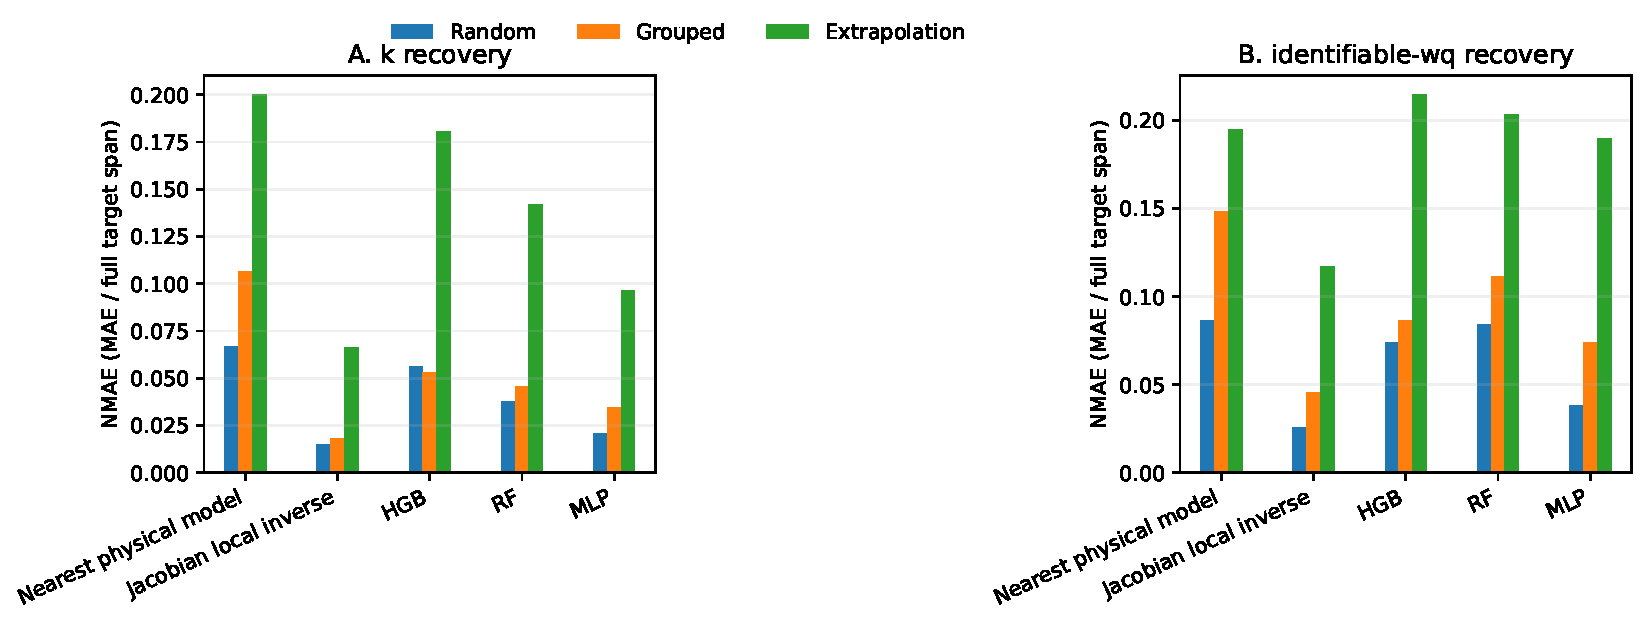
\includegraphics[width=.95\textwidth]{traditional_vs_ml_inverse.pdf}
\caption{Traditional and learned inverse methods using ringdown plus photon
geometry. Bars show median NMAE for $k$ and identifiable $\wq$ under random,
grouped, and directional protocols. The nearest and Jacobian baselines are
deterministic conditional on each registered split, whereas archived ML
summaries aggregate the existing folds and seeds. The Jacobian bars must be
read with the unclipped out-of-domain diagnostic reported in the text.}
\label{fig:mljac}
\end{figure}

Nominal 90\% conformal coverage is 0.892/0.965 for random $k/\wq$, but falls to
0.722/0.851 under grouped interpolation and 0.509/0.660 under extrapolation.
This is empirical coverage under shift, not a retained finite-sample guarantee.
Figure~\ref{fig:coverage} separates coverage by target and protocol.

\begin{figure}[tbp]
\centering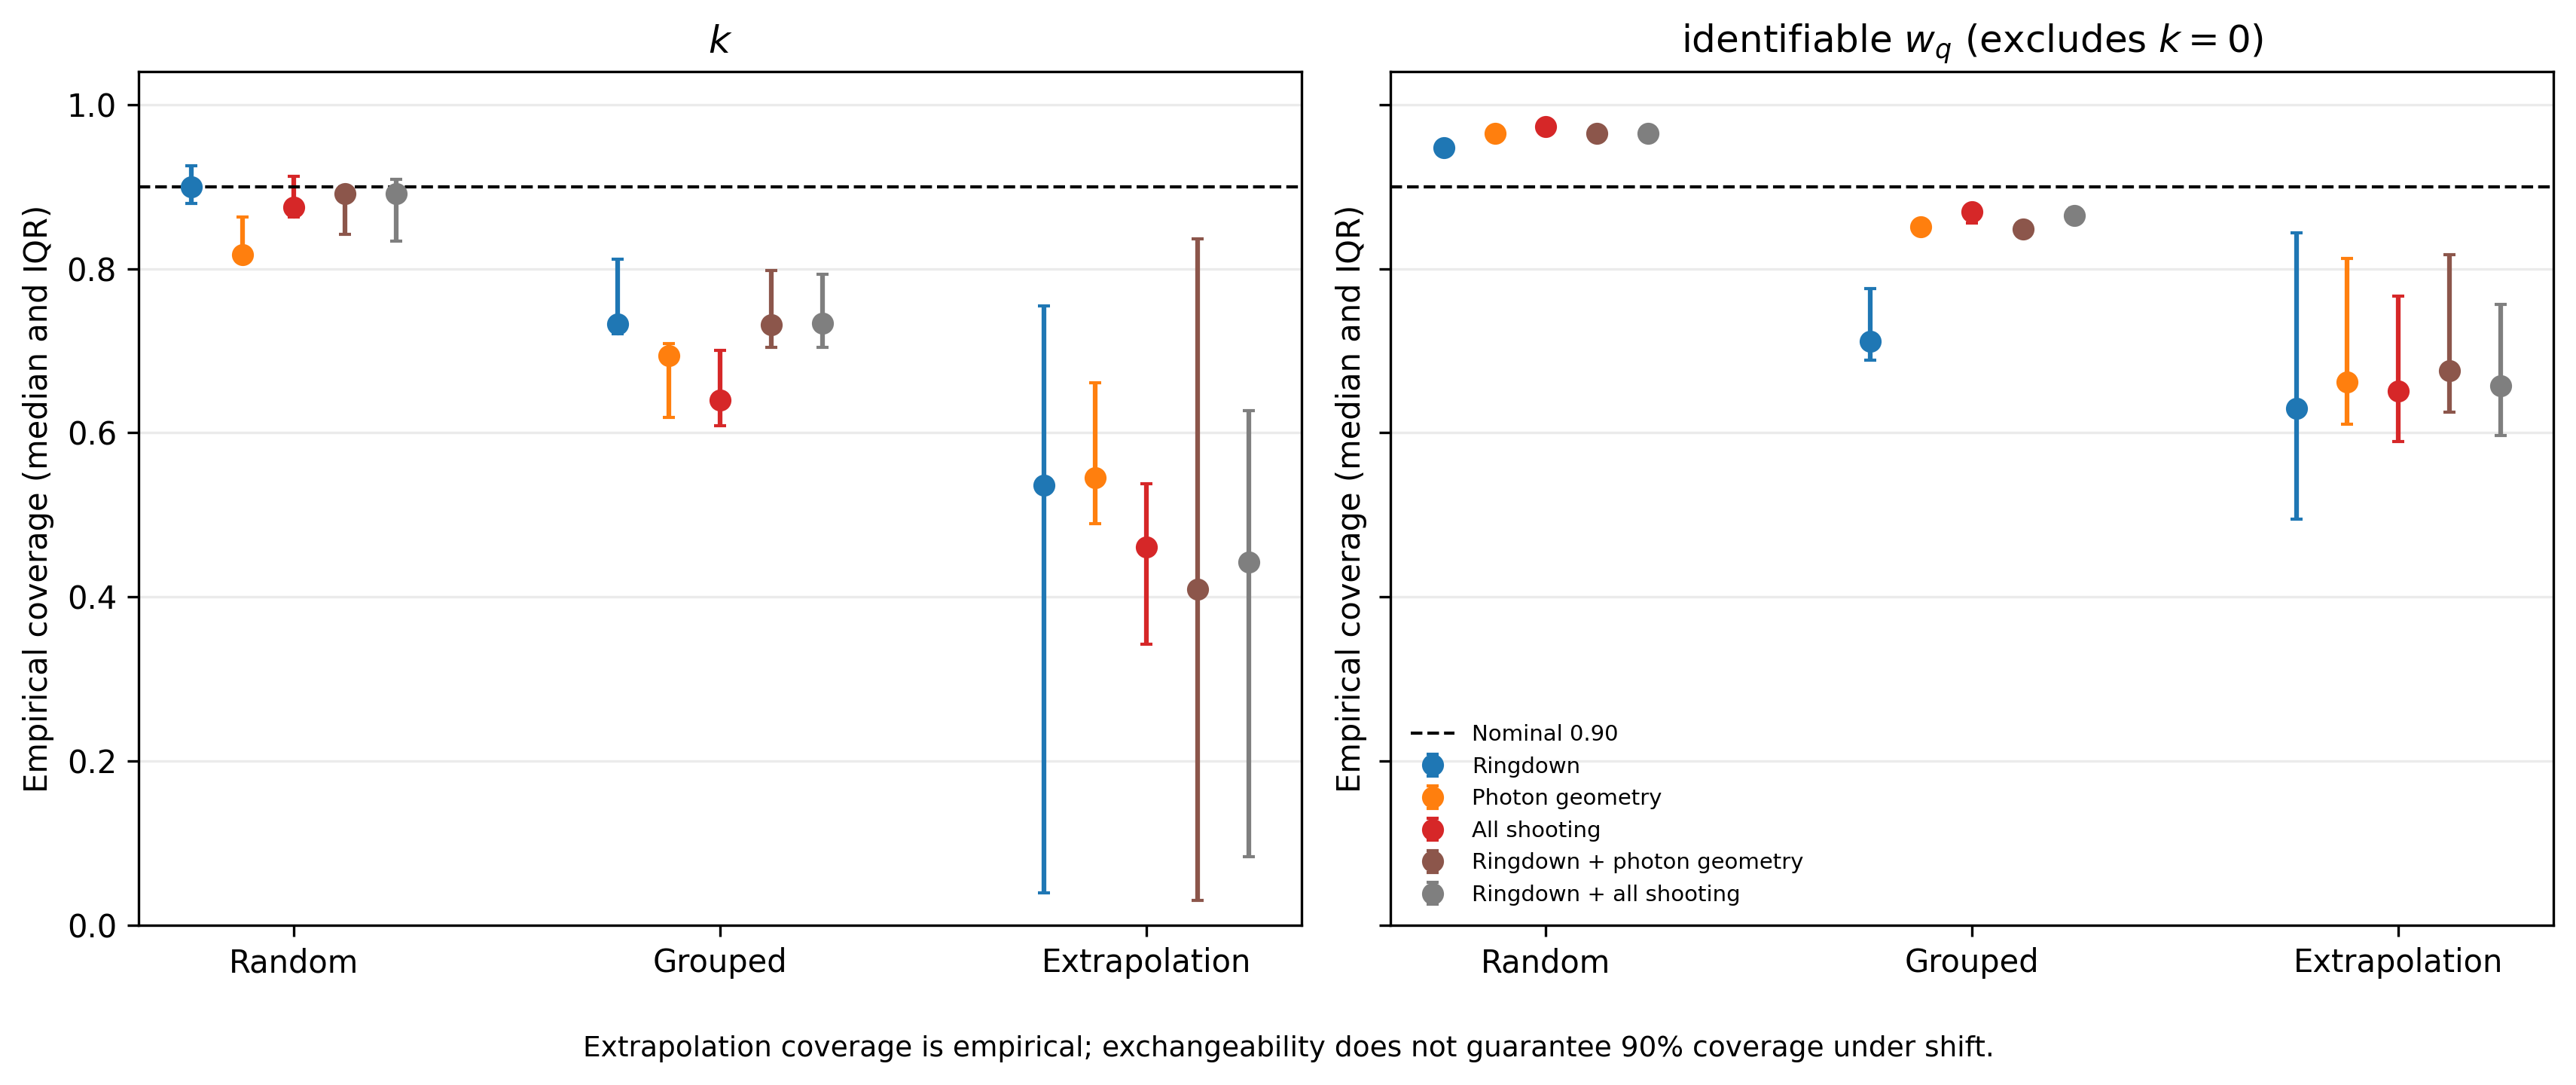
\includegraphics[width=.82\textwidth]{physical_ml_uncertainty_calibration.png}
\caption{Empirical 90\% split-conformal coverage by target and protocol.
Ordinary $\wq$ coverage excludes $k=0$; extrapolation coverage is not
guaranteed under distribution shift.}
\label{fig:coverage}
\end{figure}

\section{Numerical Convergence and Estimator Robustness}
The uniform 161-phase study completes all 121 physical points. From 9317
feature--point comparisons, 240 are unresolved under the frozen criterion;
the median normalized feature change is $7.908\times10^{-4}$ and the maximum is
0.08069. Across frozen scored predictions, the median normalized shift is
$9.482\times10^{-4}$ and the 95th percentile is 0.02606. The median aggregate
NMAE change is $6.880\times10^{-4}$, but the maximum is 16.8497 because of
unclipped MLP directional extrapolation outliers.

The targeted 321-phase audit selects 35 points deterministically before reading
their 321-phase outcomes. All complete. Median and 95th-percentile normalized
161-to-321 feature changes are $1.963\times10^{-4}$ and $7.234\times10^{-3}$;
no comparison remains unresolved, ringdown is exactly unchanged, and Jacobian
rank is preserved. Forward convergence therefore passes.
Figure~\ref{fig:resolution} displays both resolution increments on the same
selected-point order.

\begin{figure}[tbp]
\centering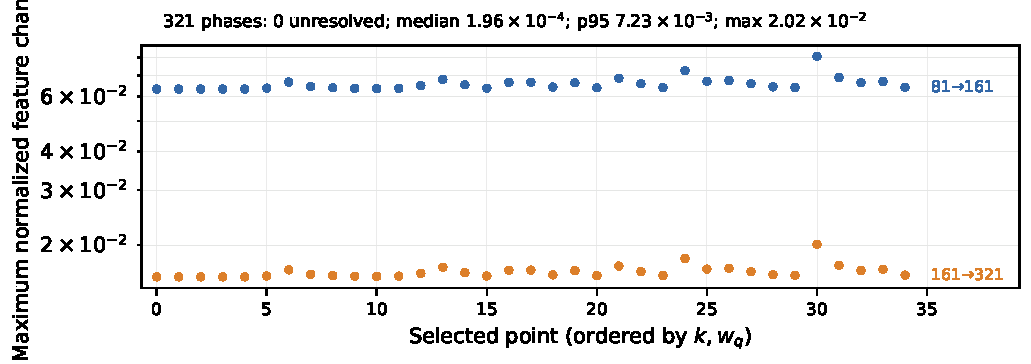
\includegraphics[width=.78\textwidth]{resolution_robustness_compact.pdf}
\caption{Targeted pointwise maximum normalized feature changes from 81 to 161
and 161 to 321 phases. The 321-phase audit resolves the forward-feature
criterion but does not by itself certify inverse estimators.}
\label{fig:resolution}
\end{figure}

Frozen trees remain tail-sensitive: HGB and RF 95th-percentile normalized
shifts are 0.08122 and 0.08509, and their largest identifiable-$\wq$ shifts are
0.30593 and 0.27053. Their median shifts are zero because many tree predictions do
not cross a split threshold. The predeclared perturbation ensembles and fixed
Extra Trees smoother do not pass all stability and grouped-performance
criteria. Of 410 catastrophic MLP records, 409 are already catastrophic at 161
phases, none is materially worsened by the 321-phase substitution, 63 reach the
iteration limit, and no numerical overflow is detected. The decision is
Outcome B: the forward map converges, but estimator robustness does not.

Typical predictions are stable, but the tails are not. The earlier MLP maxima
are not representative of every estimator, while the targeted tree failures
show that the remaining issue also cannot be attributed solely to the MLP.
The inverse-estimator robustness conclusions therefore remain conditional.

Figure~\ref{fig:estimator-robustness} separates the estimator mechanisms. Tree
medians remain exactly unchanged because most perturbations do not cross a
split, yet their tails do. The MLP reacts more smoothly to phase substitution,
while its catastrophic directional records overwhelmingly predate that
substitution.

\begin{figure}[tbp]
\centering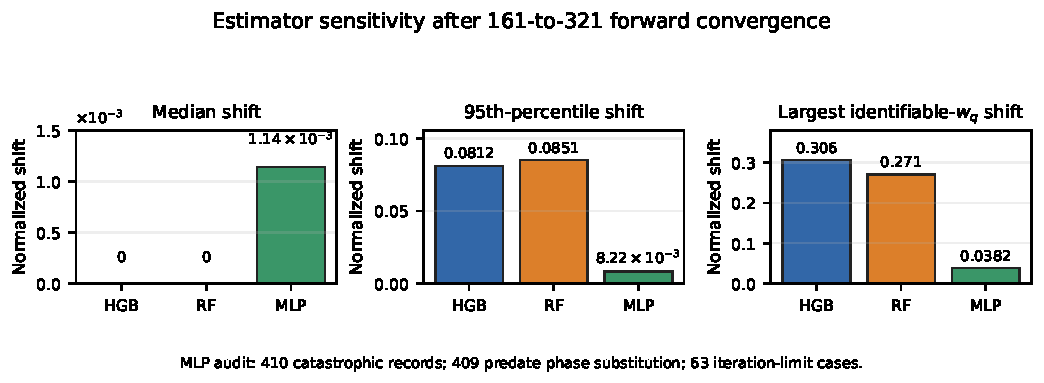
\includegraphics[width=.78\textwidth]{targeted_estimator_robustness_compact.pdf}
\caption{Frozen-estimator sensitivity after forward convergence. Bars show the
median, 95th-percentile, and largest identifiable-$\wq$ normalized prediction
shift for HGB, RF, and MLP. The audit note summarizes the distinct MLP failure
audit. No predictions are clipped.}
\label{fig:estimator-robustness}
\end{figure}

\section{Discussion}
To distinguish improved physical observability from architecture-specific
learning effects, we also evaluate non-learned nearest-model and local-linear
inverse baselines under the same physical holdout protocols. The nearest-model
improvement confirms an estimator-independent geometric contribution. Changes
in local conditioning, however, do not consistently predict pointwise recovery
across all models and protocols: Spearman associations have mixed signs and
broad bootstrap intervals. Jacobian conditioning diagnoses local physical
distinguishability, but it is not a complete predictor of finite-data error or
behavior under distribution shift, and no causal relationship is inferred.

Jacobian conditioning answers whether nearby parameter directions are separated
by the chosen observables. Training distance answers whether a fitted estimator
has support where it is evaluated. Neither statistic subsumes the other.
Consequently, $\smin$ can predict broad observable-set ordering without ranking
every empirical model or protocol.

Tree ensembles are piecewise and can show zero median response followed by
large split-crossing tails. The MLP is smoother under the targeted feature
substitution but extrapolates to physically unreasonable values in archived
directional tests. These mechanisms are estimator-specific manifestations of a
general scientific-ML risk: a converged forward simulator does not ensure a
stable inverse surrogate \cite{ovadia2019uncertainty,koh2021wilds,psaros2023uq}.

What is specific to Kiselev is the metric deformation and exact $k=0$ loss of
$\wq$. What may generalize is the workflow: establish forward rank, seek
complementary observables, partition by physical systems, test directional
shift, and perturb frozen estimators at independently measured numerical scales.

The Jacobian analysis is local by construction. The finite-grid collision
audit provides a complementary nonlocal check across the sampled parameter
domain: no unresolved distant finite-$k$ collision is found at the tested
resolution, although photon geometry rearranges local neighbor ordering.
Together with the improved nearest-model recovery, this shows that improved
distant sampled separation need not imply preservation of every local
observable-space neighborhood.

\section{Limitations}
The ringdown model is leading-eikonal rather than a dedicated finite-$\ell$
perturbative spectrum. The spacetime is static. Shooting includes only the
direct photon branch, a point emitter and point observer, and no radiative
transfer, detector response, secondary images, strain likelihood, calibration
error, or model discrepancy. The physical grid is finite. Historical proxy
results remain synthetic. Although the targeted audit resolves higher-harmonic
forward differences on its selected set, it is not a uniform 321-phase grid and
tree tail sensitivity persists. MLP extrapolation is unstable. The verdict is
therefore conditional, and no result is an observational constraint.
The finite-domain ambiguity audit does not prove continuous global injectivity;
the 121-point grid can miss isolated or continuous degeneracies between sampled
parameter values.

\section{Conclusion}
Physical complementarity is supported: ringdown constrains $k$, while photon
geometry supplies an independent direction needed for much of the $\wq$
recovery. Observable complementarity persists under a non-learned inverse
baseline, while the local Jacobian inverse demonstrates that strong local
recoverability can coexist with globally unstable predictions in this Kiselev
benchmark. Random interpolation overstates recoverability relative to grouped
and directional validation. Finally, numerical and distribution-shift audits
are necessary before confident inverse claims: the forward features can
converge while fitted estimators remain fragile. These conclusions motivate
robust inverse methods and broader physical modeling before observational use.
Within the sampled physical domain, no unresolved distant finite-$k$
observable collision is found at the tested numerical resolution, although
this finite-grid result is not a proof of continuous global identifiability.

\section*{Data Availability}
The analysis code and tracked machine-readable derived results, registered
split assignments, and reproducibility audits are available in the project
repository~\cite{palomino2026software}. This work uses simulated theoretical data and no observational
data. Large intermediate numerical products that are not tracked in the
repository are available from the author upon reasonable request.

\FloatBarrier
\appendix
\section{Historical Synthetic and Proxy Benchmark}
\label{app:historical}
The original dense benchmark used leading-eikonal curves, training-fold PCA,
and synthetic geodesic proxies. Waveform-only RF achieved
$R^2(k)=0.8960$ and $R^2(\wq)=0.9587$; HGB with proxy augmentation achieved
0.9793 and 0.9891. The rank-aware classifier reached macro F1 0.9928 with a
57.6\% weak-identifiability fraction. PCA compressed correlated information; it
did not create a new physical response direction. These historical results
motivated the physical shooting study and are not substituted for it.
Figure~\ref{fig:boundary} serves a distinct role from the historical lens in
Fig.~\ref{fig:lens}: it compares a learned rank-aware class with the analytic
weak-identifiability boundary rather than displaying conditioning or proxy
regression-error changes.

\begin{figure}[tbp]
\centering
\includegraphics[width=.65\textwidth]{learning_when_hair_is_observable_rank_aware.pdf}
\caption{Historical dense synthetic rank-aware identifiability boundary. Exact
$k=0$ rank loss is structural, whereas the finite-width weak-identifiability
region depends on precision. This historical benchmark motivated, but does not
replace, the validated physical shooting analysis.}
\label{fig:boundary}
\end{figure}

\section{Full Split Definitions}
The archived assignment table contains 115 registered split specifications
over five seeds. For each seed it contains one random interpolation split, 18
grouped splits (nine held-out blocks for each of two $3\times3$ layouts), and
four directional splits. Random splitting holds out 20\% of the 121 physical
systems for test and assigns 20\% of the remainder to calibration. The grouped
layouts use index shifts $(0,0)$ and $(1,1)$ before forming the nine contiguous
blocks; each block is held out once and 20\% of the remaining systems calibrate
the fit. Directional tests separately hold out the highest three $k$ levels,
lowest three $k$ levels, lowest three $\wq$ levels, and highest three $\wq$
levels, with 20\% of the complementary pool used for calibration. Training,
calibration, and test systems are disjoint. All $k=0$ systems remain registered;
they contribute to $k$ scoring but not ordinary $\wq$ scoring because $\wq$ is
unidentifiable there. Every scaler, noise scale, feature transform, and model
is fitted on training data only. No new split was generated for this manuscript.

\section{Feature Definitions}
Table~\ref{tab:features} lists the registered feature families. Except for the
two orbital invariants and four ringdown scalars, each phase-resolved quantity
is represented by its mean, amplitude, reference value where defined, and
sine/cosine coefficients through the third harmonic.

\begin{center}
\begin{minipage}{.96\textwidth}
\captionof{table}{Registered physical feature families and exact dimensions.}
\label{tab:features}
\centering
\scriptsize
\setlength{\tabcolsep}{3pt}
\begin{tabular}{p{.23\linewidth}p{.43\linewidth}p{.18\linewidth}r}
Family & Physical quantities & Source & Dim. \\
\hline
Ringdown & $\Delta r$, photon-sphere radius, $\Omega$, Lyapunov exponent & static metric/eikonal model & 4 \\
Orbital & radial azimuthal period, apsidal advance; summaries of $r$ and $p_r$ & timelike emitter & 20 \\
Photon geometry & summaries of impact parameter and signed sky coordinates & direct null rays & 27 \\
Redshift & summaries of photon redshift & emitter/ray/observer & 9 \\
Timing & summaries of excess delay and relative arrival time & direct null rays & 17 \\
All shooting & orbital, photon geometry, redshift, and timing & physical shooting & 73 \\
Ringdown + photon geometry & union of the corresponding families & combined & 31 \\
Ringdown + all shooting & union of the corresponding families & combined & 77 \\
\end{tabular}
\end{minipage}
\end{center}

\section{Additional Model-Level Results}
HGB and RF reproduce the central grouped photon-geometry improvement for
identifiable $\wq$. The MLP is retained as a stress test rather than omitted:
its catastrophic errors are un-clipped and included in aggregate summaries.

\section{Traditional Inverse Baselines}
\label{app:traditional}
Table~\ref{tab:traditional} gives the complete ringdown-plus-photon-geometry
comparison. Each entry is median $k$/identifiable-$\wq$ NMAE. The nearest and
local-linear methods are deterministic for a fixed registered split; their
rows are summarized over the same split assignments, while archived learned
model rows retain the existing fold/seed aggregation.

\begin{center}
\begin{minipage}{.82\textwidth}
\captionof{table}{Traditional and learned inversion with ringdown plus photon
geometry. NMAE is MAE divided by the full target span; $k=0$ remains in $k$
scoring but is excluded from identifiable-$\wq$ scoring.}
\label{tab:traditional}
\centering
\small
\begin{tabular}{lccc}
Method & Random & Grouped & Directional \\
\hline
Nearest physical model & 0.0667/0.0866 & 0.1063/0.1481 & 0.2000/0.1950 \\
Local Jacobian inverse & 0.0147/0.0259 & 0.0184/0.0454 & 0.0661/0.1172 \\
HGB & 0.0560/0.0740 & 0.0530/0.0865 & 0.1803/0.2146 \\
RF & 0.0378/0.0844 & 0.0457/0.1113 & 0.1418/0.2033 \\
MLP & 0.0206/0.0383 & 0.0344/0.0738 & 0.0966/0.1896 \\
\end{tabular}
\end{minipage}
\end{center}

The primary Jacobian predictions are raw and unclipped: 1315 of 9950 fall
outside $0\leq k\leq0.0025$ or $-0.7125\leq\wq\leq-0.45$. Reference
condition number, reference $\smin$, and local observable-space distance are
stored for every prediction. Figure~\ref{fig:conditioning-recovery} reports the
supported pointwise/fold-level conditioning analysis. Most bootstrap intervals
span zero, and the significant nearest-model associations are negative; these
mixed results reinforce that local conditioning is not a complete
estimator-error model.

\begin{center}
\begin{minipage}{.76\textwidth}
\centering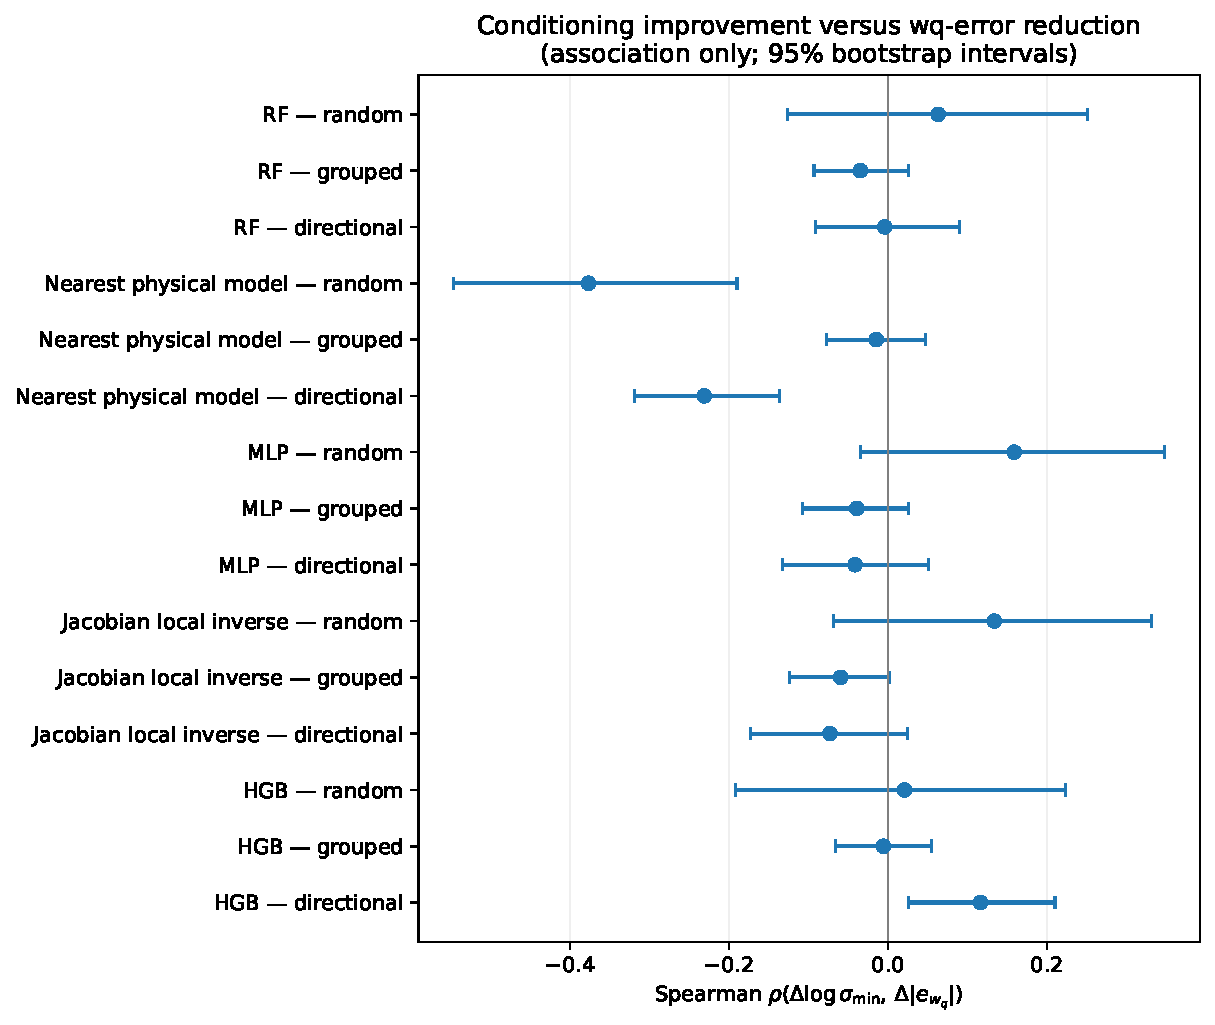
\includegraphics[width=.92\linewidth]{conditioning_vs_wq_recovery.pdf}
\captionof{figure}{Spearman association between the change in log minimum singular value
and the reduction in absolute identifiable-$\wq$ error when photon geometry is
added to ringdown. Points show method/protocol estimates and bars are 95\%
bootstrap intervals. Associations are descriptive and do not imply causation.}
\label{fig:conditioning-recovery}
\end{minipage}
\end{center}

\section{Four Directional Extrapolation Tests}
Directions are stored independently in the prediction tables before any median
summary. High-to-low and low-to-high tests differ in training support and cannot
be interpreted as interchangeable folds.

\section{Conformal Calibration and Rejection}
Split-conformal residual quantiles are fitted on calibration subsets. The
exchangeability guarantee applies to matching distributions; shifted coverage
is reported empirically. Rejection curves rank uncertainty but do not repair
distribution shift.

\section{Noise and Learning Curves}
Grouped one-percent feature noise yields ringdown-plus-photon-geometry NMAE
0.0699/0.0853 for $k/\wq$. Learning curves are still improving at 78 training
points, so data limitation remains part of the interpretation.

\section{Numerical-Validation Thresholds}
\label{app:numerical-thresholds}
The 35-point 321-phase run takes 5318.2 s. Maximum hit, timelike-constraint,
null-constraint, and impact-parameter drift errors are respectively
$7.0913\times10^{-8}$, $3.1303\times10^{-13}$,
$7.6214\times10^{-12}$, and $1.7932\times10^{-11}$.
The Schwarzschild arrival-time comparison in Fig.~\ref{fig:schwarzschild}
separates the visually overlapping phase-resolved series from their actual-scale residuals.

\begin{figure}[tbp]
\centering

\includegraphics[width=.62\textwidth]{schwarzschild_arrival_validation_with_residuals.pdf}
\caption{Schwarzschild arrival-time validation. Four arrival-time phase-resolved series are
plotted. The two nominal $\wq$ cases coincide because the $k=0$ geometry is
Schwarzschild, while the direct and integrated-redshift constructions agree
within numerical quadrature error. The lower panel shows direct minus
integrated arrival time for $w_q=-0.5$ and the direct-arrival difference
between $w_q=-0.5$ and $w_q=-2/3$ on their actual numerical scales.}
\label{fig:schwarzschild}
\end{figure}

Matched Schwarzschild and Kiselev direct rays are compared on their actual
coordinate scale in Fig.~\ref{fig:ray-difference}.

\begin{center}
\begin{minipage}{.90\textwidth}
\centering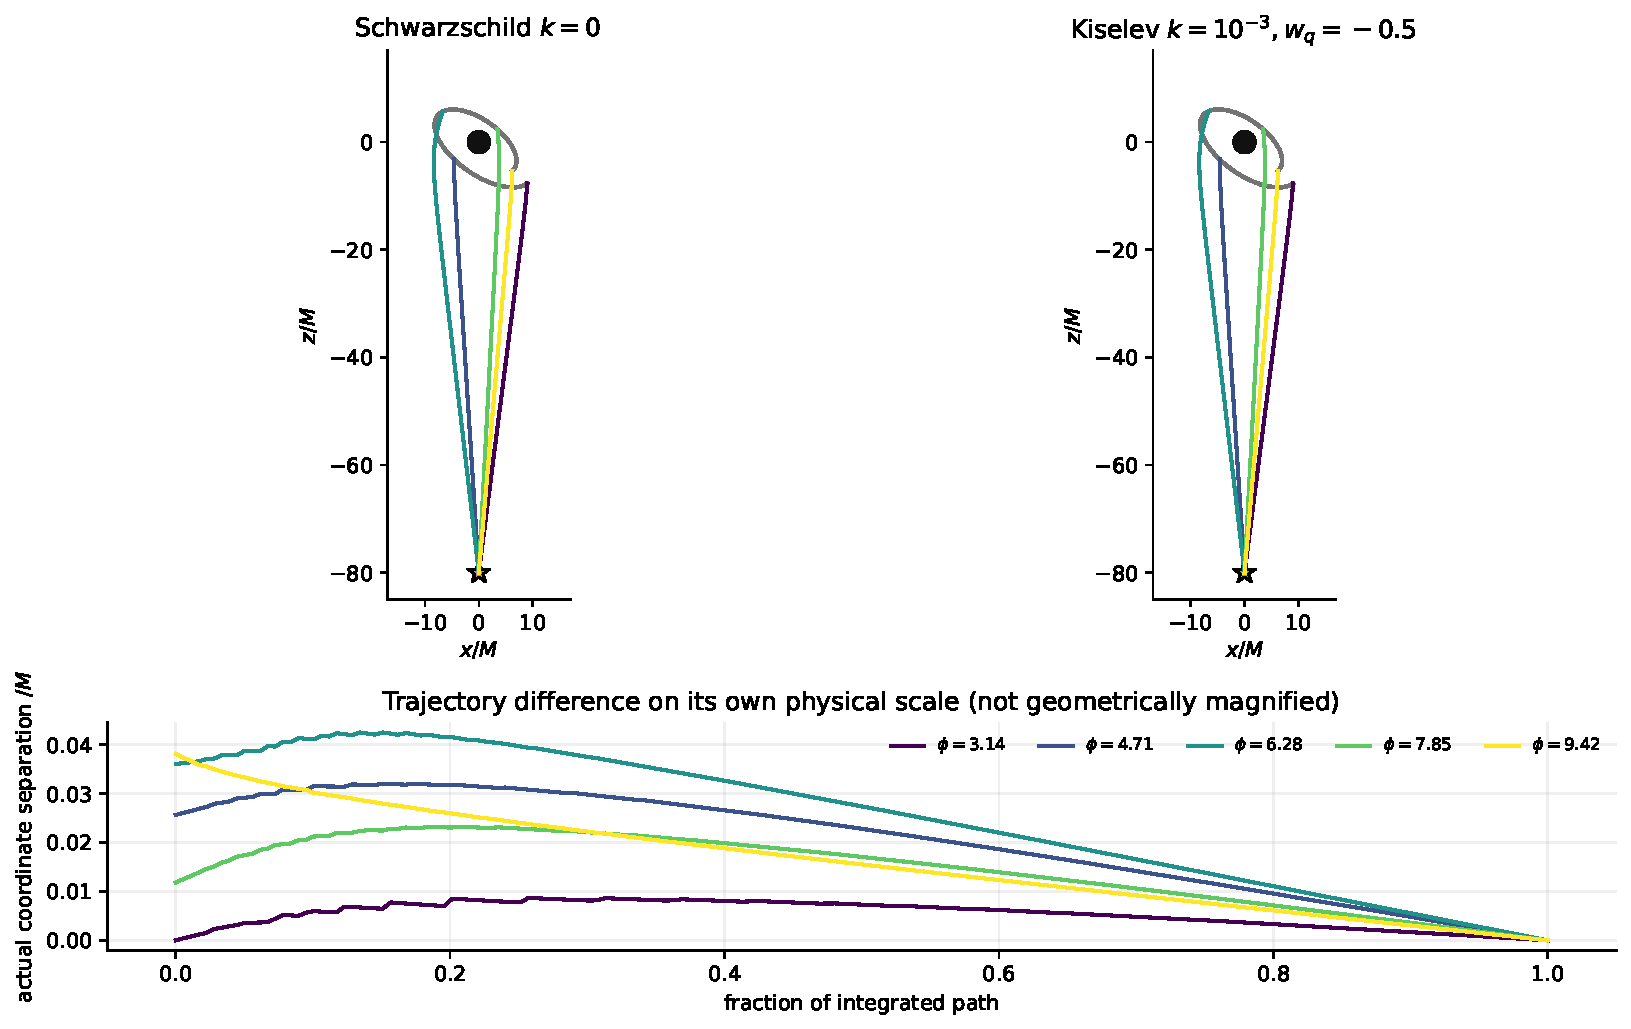
\includegraphics[width=.96\linewidth]{shooting/schwarzschild_kiselev_ray_comparison.pdf}
\captionof{figure}{Matched-phase direct rays for Schwarzschild and $k=10^{-3}$,
$w_q=-0.5$ with $M=1$, $r_p=8M$, $r_a=12M$, and observer $(0,0,-80M)$. The
lower panel gives physical coordinate separation versus integrated path
fraction. Differences are shown on their actual scale and are not
geometrically magnified.}
\label{fig:ray-difference}
\end{minipage}
\end{center}

\section{Uniform 161-Phase Convergence Audit}
All 121 points complete in 4473.2 s with zero failed points. The audit preserves
the exact $k=0$ boundary and uses no mixed-resolution row, interpolation, or
proxy substitution.

\section{Reproducibility Summary}
The physical grid contains 121 points. The uniform 161-phase audit completed
all points, and the targeted 321-phase audit completed all 35 preselected
points. Exact $k=0$ rank loss is preserved. Registered split assignments are
reused, preprocessing is fitted on training data only, and the traditional
inverse numerical audit passed. The independent physics audit passed with the
launch-angle warning documented below.

\section{Independent Physical-Shooting Audit}
The independent reference implementation imported no production
\texttt{bhhairml} physics code and compared against archived production
outputs rather than rerunning the full 321-phase campaign. Invariant launch
directions, rays, observer-plane hits, physical observables, extracted features,
and selected Jacobians agree. The verdict is \texttt{PASS\_WITH\_WARNING}: raw
launch angles need not be unique because equivalent angular branches encode
the same unit direction and physical ray. Raw angle equality is therefore not
a required invariant, and the warning is not a physics discrepancy.

\section{Finite-Domain Observable-Ambiguity Audit}
\label{app:ambiguity}
This audit evaluates all pairwise distances on the registered 121-point
physical grid. It cannot rule out isolated or continuous degeneracies between
sampled points and therefore does not establish continuous global injectivity.
For points $i,j$, normalized parameter separation is
\begin{equation}
d_\theta(i,j)=\sqrt{\left(\frac{k_i-k_j}{\Delta k}\right)^2+
\left(\frac{w_{q,i}-w_{q,j}}{\Delta w_q}\right)^2},
\end{equation}
where both spans are taken from the registered physical domain. Observable
differences use the archived grid-wide q95--q05 feature scales. The primary
cross-set distance is the RMS of standardized feature differences rather than
a raw Euclidean norm, because the combined set has 31 dimensions while
ringdown has four.

At $k=0$, the ringdown distance across all 55 nominal-$\wq$ pairs is exactly
zero. For ringdown plus photon geometry the minimum and median are zero and the
maximum is $2.63\times10^{-12}$. This is the required positive control and
reproduces the exact Schwarzschild structural degeneracy to numerical
precision; these pairs are not counted as undesirable collisions.

\begin{center}
\begin{minipage}{.88\textwidth}
\captionof{table}{Closest finite-$k$ RMS standardized observable pair at each
minimum normalized parameter separation.}
\label{tab:ambiguity-thresholds}
\centering
\small
\begin{tabular}{lrrrr}
Feature set & $d_\theta\geq0.10$ & $\geq0.25$ & $\geq0.50$ & $\geq0.75$ \\
\hline
Ringdown & 0.005832 & 0.012668 & 0.025170 & 0.041655 \\
Rdown + photon geom. & 0.007710 & 0.013406 & 0.031550 & 0.072741 \\
\end{tabular}
\end{minipage}
\end{center}

\begin{figure}[tbp]
\centering
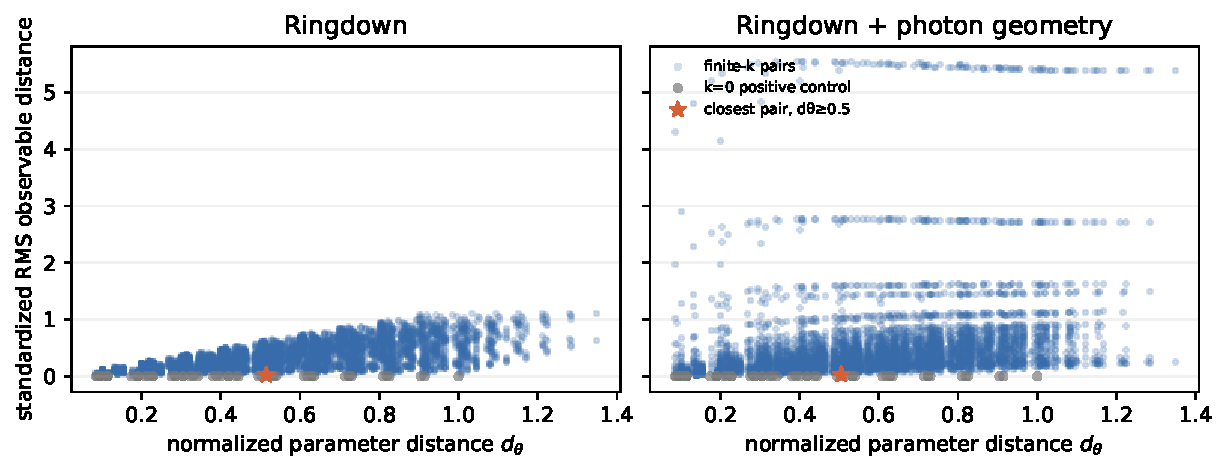
\includegraphics[width=.88\textwidth]{finite_domain_global_ambiguity.pdf}
\caption{All-pairs finite-domain ambiguity audit. The horizontal axis is
normalized parameter distance and the vertical axis is RMS standardized
observable distance. Grey $k=0$ pairs show the required structural degeneracy;
distant finite-$k$ pairs are the relevant sampled-domain diagnostic. Stars mark
the closest finite-$k$ pair with $d_\theta\geq0.5$. This plot tests only the
sampled physical grid and does not establish continuous global injectivity.}
\label{fig:finite-ambiguity}
\end{figure}

\begin{center}
\begin{minipage}{.96\textwidth}
\captionof{table}{Nearest-observable-neighbor parameter distance and
preservation of the nearest parameter-space neighbor. Poorer exact local
neighbor preservation does not imply increased distant ambiguity.}
\label{tab:ambiguity-neighbors}
\centering
\scriptsize
\begin{tabular}{lrrrrrr}
Feature set & median $d_\theta$ & p90 & max. & top-1 & top-3 & top-5 \\
\hline
Ringdown & 0.09524 & 0.21513 & 0.23216 & 40.9\% & 71.8\% & 75.5\% \\
Rdown + photon geom. & 0.13171 & 0.21759 & 0.21886 & 20.0\% & 48.2\% & 67.3\% \\
\end{tabular}
\end{minipage}
\end{center}

No nearest observable neighbor lies beyond $d_\theta=0.25$ for either set,
and no pair with $d_\theta\geq0.25$ lies below the fifth-percentile local
spacing. The closest combined pair at $d_\theta\geq0.5$ is 12.8 times the
largest measured combined-feature 161-to-321 RMS change. Photon geometry
improves the distant-pair diagnostics but not every local ordering statistic.

\section{MLP Extrapolation-Failure Audit}
The machine-readable table contains standardized input magnitude, hidden
activation magnitude, iteration status, overflow flag, training distance, and
resolution response for every catastrophic record. It distinguishes
optimization failure from extrapolation instability without clipping.

Exact frozen-estimator shift summaries used in
Fig.~\ref{fig:estimator-robustness} are retained in
Table~\ref{tab:robustness} for numerical reference.

\begin{center}
\begin{minipage}{.72\textwidth}
\captionof{table}{Targeted 321-phase frozen-estimator robustness.}
\label{tab:robustness}
\centering
\begin{tabular}{lccc}
Model & median & 95th percentile & max. $\wq$ \\
\hline
HGB & 0 & 0.08122 & 0.30593 \\
RF & 0 & 0.08509 & 0.27053 \\
MLP & 0.001143 & 0.008223 & 0.03819 \\
\end{tabular}
\end{minipage}
\end{center}

\FloatBarrier
\bibliographystyle{plain}
\bibliography{references}
\end{document}
